\section{Experimental results}
In this section finally discusses results of actual flight tests.
The task for the experiments is to track different reference trajectories while using the same controller and parameter values.
As the tracking errors for the following experiments were small, there was no distinguishable difference between the particle, body and energy based approaches.
The data for the presented figures were recorded while using the body based control approach.

The controller parameters for the following experiments are summarized in \autoref{tab:ParamTriQuadCtrl}.
Note that the values for inertia etc.\ are w.r.t.\ the body fixed frame and not w.r.t.\ the (closed loop) center of mass as done in \autoref{sec:CtrlExampleQuadcopter}.
Consequently the some values differ from what the matching conditions in \eqref{eq:CtrlExampleQuatMatchedParam} would suggest.

\begin{table}
 \centering
 \setlength{\tabcolsep}{.1em}
 \begin{tabular}{crlrll}
  \toprule
  \phantom{|} \quad symbol \quad\phantom{|} & \multicolumn{2}{c}{\phantom{|} \quad tricopter value \quad\phantom{|} } & \multicolumn{2}{c}{\phantom{|} \quad quadcopter value \quad\phantom{|}} & \multicolumn{1}{c}{\phantom{|} \qquad comment \qquad\phantom{|}} \\
  \midrule
  $\Ts$  & \multicolumn{4}{c}{$0.005\,\unit{s}$} & main sampling time \\
  \midrule
  $\quad\mc\quad$ & \phantom{|} \qquad$1.251$&$\unit{kg}$ & \phantom{|} \qquad$1.001$&$\unit{kg}$ & same as model \\
  $\scz$ & $ 0 $&$\unit{m}$ & $ 0.043$&$\unit{m}$ & center of mass \\
  $\Jcxx=\Jcyy$ & $0.0192$&$\unit{kg}\,\unit{m}^2$& $0.0095$&$\unit{kg}\,\unit{m}^2$ & tilt inertia \\
  $\Jczz$ & $0.0308$&$\unit{kg}\,\unit{m}^2$ & $0.0307$&$\unit{kg}\,\unit{m}^2$ & same as model 
  \\[.3ex]
  $\quad\dc\quad$ & $6$&$\tfrac{\unit{kg}}{\unit{s}}$ & $4.4$&$\tfrac{\unit{kg}}{\unit{s}}$ & translation damping \\
  $\lcz$ & $ 0 $&$\unit{m}$ & $ 0.255$&$\unit{m}$ & center of damping \\
  $\sigcxx=\sigcyy$ & $0.3$&$\tfrac{\unit{kg}\,\unit{m}^2}{\unit{s}}$& $0.4$&$\tfrac{\unit{kg}\,\unit{m}^2}{\unit{s}}$ & tilt damping \\
  $\sigczz$ & $0.25$&$\tfrac{\unit{kg}\,\unit{m}^2}{\unit{s}}$ & $0.1$&$\tfrac{\unit{kg}\,\unit{m}^2}{\unit{s}}$ & yaw damping
  \\[.3ex]
  $\quad\kc\quad$ & $8$&$\tfrac{\unit{kg}}{\unit{s}^2}$ & $8$&$\tfrac{\unit{kg}}{\unit{s}^2}$ & translation stiffness \\
  $\hcz$ & $ 0 $&$\unit{m}$ & $ 0.255$&$\unit{m}$ & center of stiffness \\
  $\kapcxx=\kapcyy$ & $1.7$&$\tfrac{\unit{kg}\,\unit{m}^2}{\unit{s}}$& $2.6$&$\tfrac{\unit{kg}\,\unit{m}^2}{\unit{s}}$ & tilt stiffness \\
  $\kapczz$ & $0.7$&$\tfrac{\unit{kg}\,\unit{m}^2}{\unit{s}}$ & $0.2$&$\tfrac{\unit{kg}\,\unit{m}^2}{\unit{s}}$ & yaw stiffness \\
  \midrule
  $\PropObsGainVel$  & \multicolumn{4}{c}{$0.1$} & propeller obs.\ gain 1 \\
  $\PropObsGainBias$  & \multicolumn{4}{c}{$0.01\,\unit{Hz}$} & propeller obs.\ gain 2 \\
  $\PropCtrlGain$  & \multicolumn{4}{c}{$0.25$} & propeller control gain \\
  $c_F$ & $0.1$& & & & thrust filter param \\
  $\omega_{\mathsf{mag}}$ & & & $100$&$\tfrac{\unit{RAD}}{\unit{s}}$ & thrust mag.\ bandw.\ \\
  $\zeta_{\mathsf{mag}}$ & & & $0.707$& & thrust mag.\ damp.\ ratio \\
  $\omega_{\mathsf{tilt}}$ & & & $125$&$\tfrac{\unit{RAD}}{\unit{s}}$ & tilt torque bandw.\ \\
  $\zeta_{\mathsf{tilt}}$ & & & $0.707$& & tilt torque damp.\ ratio \\
  $\omega_{\mathsf{head}}$ & & & $66$&$\tfrac{\unit{RAD}}{\unit{s}}$ & head.\ torque bandw.\ \\
  \midrule
  $L_\omega$  & \multicolumn{4}{c}{$0.2$} & ang.\ vel.\ obs.\ gain \\
  $L_\tau$  & \multicolumn{4}{c}{$0.01$} & torque bias obs.\ gain \\
  $\cTPC$  & \multicolumn{4}{c}{$0.99$} & clock offset estimator root \\
  $l_r$  & \multicolumn{4}{c}{$1$} & pos.\ obs.\ fb.\ gain 1 \\
  $l_v$  & \multicolumn{4}{c}{$0.575$} & pos.\ obs.\ fb.\ gain 2 \\
  $l_a$  & \multicolumn{4}{c}{$-0.025$} & pos.\ obs.\ fb.\ gain 3 \\
  $l_F$  & \multicolumn{4}{c}{$0.01$} & force bias obs.\ fb.\ gain \\
  \bottomrule
 \end{tabular}
 \caption{Parameter values for tri- and quadcopter controller}
 \label{tab:ParamTriQuadCtrl}
\end{table}


\paragraph{Error quantization.}
In order to quantify the tracking performance we use the scalar quantities 
%position error $e_{\r}$, attitude error $e_{\R}$ and heading error $e_{\head}$ defined as
\begin{subequations}
\begin{align}
 e_{\r} &= \norm{\rObs - \rR},
\\
 e_{\R} &= \cos^{-1} \big( \tfrac{1}{2} (\tr\RE - 1) \big), \quad \RE = \RRT \RObs,
\\
 e_{\head} &= |\atanTwo(\REyx - \RExy, \RExx + \REyy)|.
\end{align} 
\end{subequations}
The position error $e_{\r}$ is the Euclidean distance between estimated position $\rObs$ and its reference $\rR$.
The attitude error $e_{\R}$ is the angle of the rotation matrix $\RE$ which rotates the reference attitude $\RR$ to the estimated attitude $\RObs$.
The heading error $e_{\head}$ is roughly the yaw angle of the error attitude $\RE$.

There are two reasons for considering the heading error $e_{\head}$ in addition to the attitude error $e_{\R}$:
Firstly the copters behave differently for the tilting degree of freedom and the heading.
This is also reflected by the different controller parameters for the respective directions.
Secondly, for the quadcopter, the tilting is used to compensate a horizontal position error.
A horizontal bias force implies a tilt error and consequently an attitude error.
%Based on the arguments from \autoref{sec:RealizationRefGenFlatness} one could say that the heading error $e_{\head}$ captures the part of the attitude error that is ``orthogonal'' to the tilt error.
Note that there is the relation $e_{\R} \geq e_{\head}$.

To quantify the errors for an experiment containing $N$ sampling steps we use the root-mean-square
\begin{align}
 \RMS(e_{\r}) = \sqrt{ \tfrac{1}{N} \textstyle{\sum_{k=1}^{N} \big( e_{\r}[k] \big)^2} }.
\end{align}
As an indicator for the dynamic of the reference trajectory for one experiment we consider the maximal velocity
\begin{align}
 \max(\norm{\vR}) = \max\big( \norm{\vR[1]}, \ldots, \norm{\vR[N]} \big)
\end{align}
and in the same way the maximal acceleration $\max(\norm{\vRd})$, the maximal angular velocity $\max(\norm{\wR})$ and the maximal angular acceleration $\max(\norm{\wRd})$.

The resulting values for the following four experiments are collected in \autoref{tab:MulticopterExperimentStatistics}.
Evidently, the quadcopter experiments are much more dynamic.
This is due to the fact that the quatcopter has a much better thrust to mass and torque to inertia ratio.

\begin{table}[htb]
 \centering
 \setlength{\tabcolsep}{.1em}
 \begin{tabular}{rlcccc}
  \toprule
   && \quad tricopter\quad & \quad quadcopter\quad & \quad quadcopter\quad & \quad quadcopter\quad \\
   && \quad transitions \quad & \quad transitions \quad & \quad looping \quad & \quad flip \quad \\
  \midrule
  $\max(\norm{\vR})$  &in $\tfrac{\unit{m}}{\unit{s}}$     & $2.2$   & $3.4$   & $4.2$   & $2.3$ \\[.5ex]
  $\max(\norm{\vRd})$ &in $\tfrac{\unit{m}}{\unit{s}^2}$   & $3.9$   & $8.2$   & $17.1$   & $17.5$ \\[.5ex]
%  $\max(\norm{\vRd})$ &in $\tfrac{\unit{m}}{\unit{s}^2}$   & $5.0$   & $8.2$   & $4.9$   & $7.8$ \\[.5ex]
  $\max(\norm{\wR})$  &in $\tfrac{\unit{deg}}{\unit{s}}$   & $318$   & $271$   & $537$   & $736$ \\[.5ex]
  $\max(\norm{\wRd})$ &in $\tfrac{\unit{deg}}{\unit{s}^2}$ & $497$   & $1380$  & $1610$  & $2480$ 
  \\[1ex]
  $\RMS(e_{\r})$      &in $\unit{m}$                       & $0.013$ & $0.017$ & $0.027$ & $0.026$ \\[.5ex]
  $\RMS(e_{\R})$      &in $\unit{deg}$                     & $1.1$   & $1.3$   & $2.5$   & $2.1$   \\[.5ex]
  $\RMS(e_{\head})$   &in $\unit{deg}$                     & $0.95$  & $0.3$   & $1.2$   & $0.8$   \\
  \bottomrule
 \end{tabular}
 \caption{Statistical values for the multicopter experiments}
 \label{tab:MulticopterExperimentStatistics}
\end{table}


\paragraph{Tricopter transitions.}
\autoref{fig:TriManeuver42Result} shows measurements of the tricopter tracking polynomial transitions between constant configurations.
A video of this experiment is available here\footnote{\url{https://youtu.be/oS5PHr6H0K4}}.

In the first $10\,\unit{s}$ the tricopter does some horizontal movement while maintaining the attitude and height.
For the next $10\,\unit{s}$ it tracks similar trajectories, but this time using the body tilt to generate the necessary horizontal force.
The difference between the approaches is obvious in the trajectories for the servo angles for the first case and the roll and pitch angle for the second case.
Furthermore a $90^\circ$ heading transition is added to the last two position transitions.
In the last third of the maneuver the tricopter tilts while maintaining its position.
One can see that for a body tilt of $15^\circ$ the servos have to tilt more than $30^\circ$.
The last transition is a $360^\circ$ heading rotation and $1\,\unit{m}$ height transition in $2\,\unit{s}$.
This is the part where we have the maximal attitude error of about $5^\circ$.
Here in particular one can see that the heading error $e_{\head}$ is the mayor part of the attitude error $e_{\R}$.

Comparing the performance of this tricopter experiment with the following quadcopter experiments, see \autoref{tab:MulticopterExperimentStatistics}, one can see that the tricopter has the lowest position and attitude error.
However, the comparison is not really fair since the quadcopter trajectories are much more dynamic.

\paragraph{Quadcopter transitions.}
\autoref{fig:QuadManeuver42Result} shows measurements of the quadcopter tracking polynomial transitions between constant configurations.
A video of this and the following experiments is available here\footnote{\url{https://youtu.be/x66sua3M6RQ}}.

The reference trajectories are very similar to the previous transitions for the tricopter, but with reduced transitions times.
The maximal velocity and acceleration, see \autoref{tab:MulticopterExperimentStatistics}, are achieved at about $12\,\unit{s}$, for a $2\,\unit{m}$ horizontal transition in $1.5\,\unit{s}$.
Since the tilt here is almost $45^\circ$ it is evident that the acceleration must be almost $\norm{\gravityAcc}$.
The last transition is a $360^\circ$ heading rotation in $4\,\unit{s}$, which is much slower as the corresponding maneuver for the tricopter due to the limited control torque of the quadcopter.
On the other hand the heading error $e_{\head}$ during this maneuver is much better as with the tricopter.
This might be a positive result of the sophisticated thrust controller from \autoref{sec:RealizationForceVectorControl}.

\paragraph{Quadcopter looping.}
\autoref{fig:QuadLoopResult} shows measurements of the quadcopter tracking four looping trajectories.
The reference trajectory for $\rx$ and $\rz$ is essentially a vertical circle with $2\,\unit{m}$ diameter, see \autoref{fig:introQuadLoopSnapshots}.
The individual looping takes about $3\,\unit{s}$ from rest to rest.

This is the first maneuver which involves that the quadcopter is upside down, i.e.\ $\RR \ez = -\ez$, so an appropriate method for the heading reference generation is required here.
Though the accelerations are quite high as well, this experiment has in comparison to the the others the highest translational velocity.
The fact that it has largest position and attitude errors could suggest that there are large model errors and/or unknown disturbances related to higher translational velocity.

% \begin{figure}
%  \centering
%  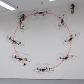
\includegraphics[width=.6\linewidth]{graphics/QuadLoopSnapshots.png}
%  \caption{Snapshots of the quadcopter tracking the loop trajectory}
%  \label{fig:QuadLoopSnapshots}
% \end{figure}

\paragraph{Quadcopter flip.}
\autoref{fig:QuadFlipResult} shows measurements of the quadcopter tracking six flip trajectories about different axis.
A flip is a trajectory where the quadcopter does a $360^\circ$ tilt transition while trying to minimize translational movement.
The maneuver here requires a vertical clearance of less than $1\,\unit{m}$ and just a few centimeters horizontally.
The individual flip takes less than $2\,\unit{s}$ from rest to rest.

This maneuver contains the largest translational and angular accelerations of the four experiments.
The maximal linear acceleration of $17.5\,\tfrac{\unit{m}}{\unit{s}^2}$ obviously appears when the quadcopter is upside down.
Here gravity pulls it with $9.81\,\tfrac{\unit{m}}{\unit{s}^2}$ and the propellers generate significant thrust in the same direction.

\begin{figure}
 \centering
 \includegraphics{graphics/TriFlightTest/TriManeuver42Result}
 \caption{Tricopter flight test result for polynomial transition trajectories}
 \label{fig:TriManeuver42Result}
\end{figure}

\begin{figure}
 \centering
 \includegraphics{graphics/QuadFlightTest/QuadManeuver42Result}
 \caption{Quadcopter flight test result for polynomial transition trajectories}
 \label{fig:QuadManeuver42Result}
\end{figure}

\begin{figure}
 \centering
 \includegraphics{graphics/QuadFlightTest/QuadLoopResult}
 \caption{Quadcopter flight test result for looping trajectories}
 \label{fig:QuadLoopResult}
\end{figure}

\begin{figure}
 \centering
 \includegraphics{graphics/QuadFlightTest/QuadFlipResult}
 \caption{Quadcopter flight test result for the flip trajectories}
 \label{fig:QuadFlipResult}
\end{figure}